Первый вариант архитектуры модуля \texttt{remap}, содержащий специальный модуль синхронизации тактовых доменов, представлен на рисунке \ref{fig:remap_cds}.\par
\begin{figure}[ht]
    \centering
    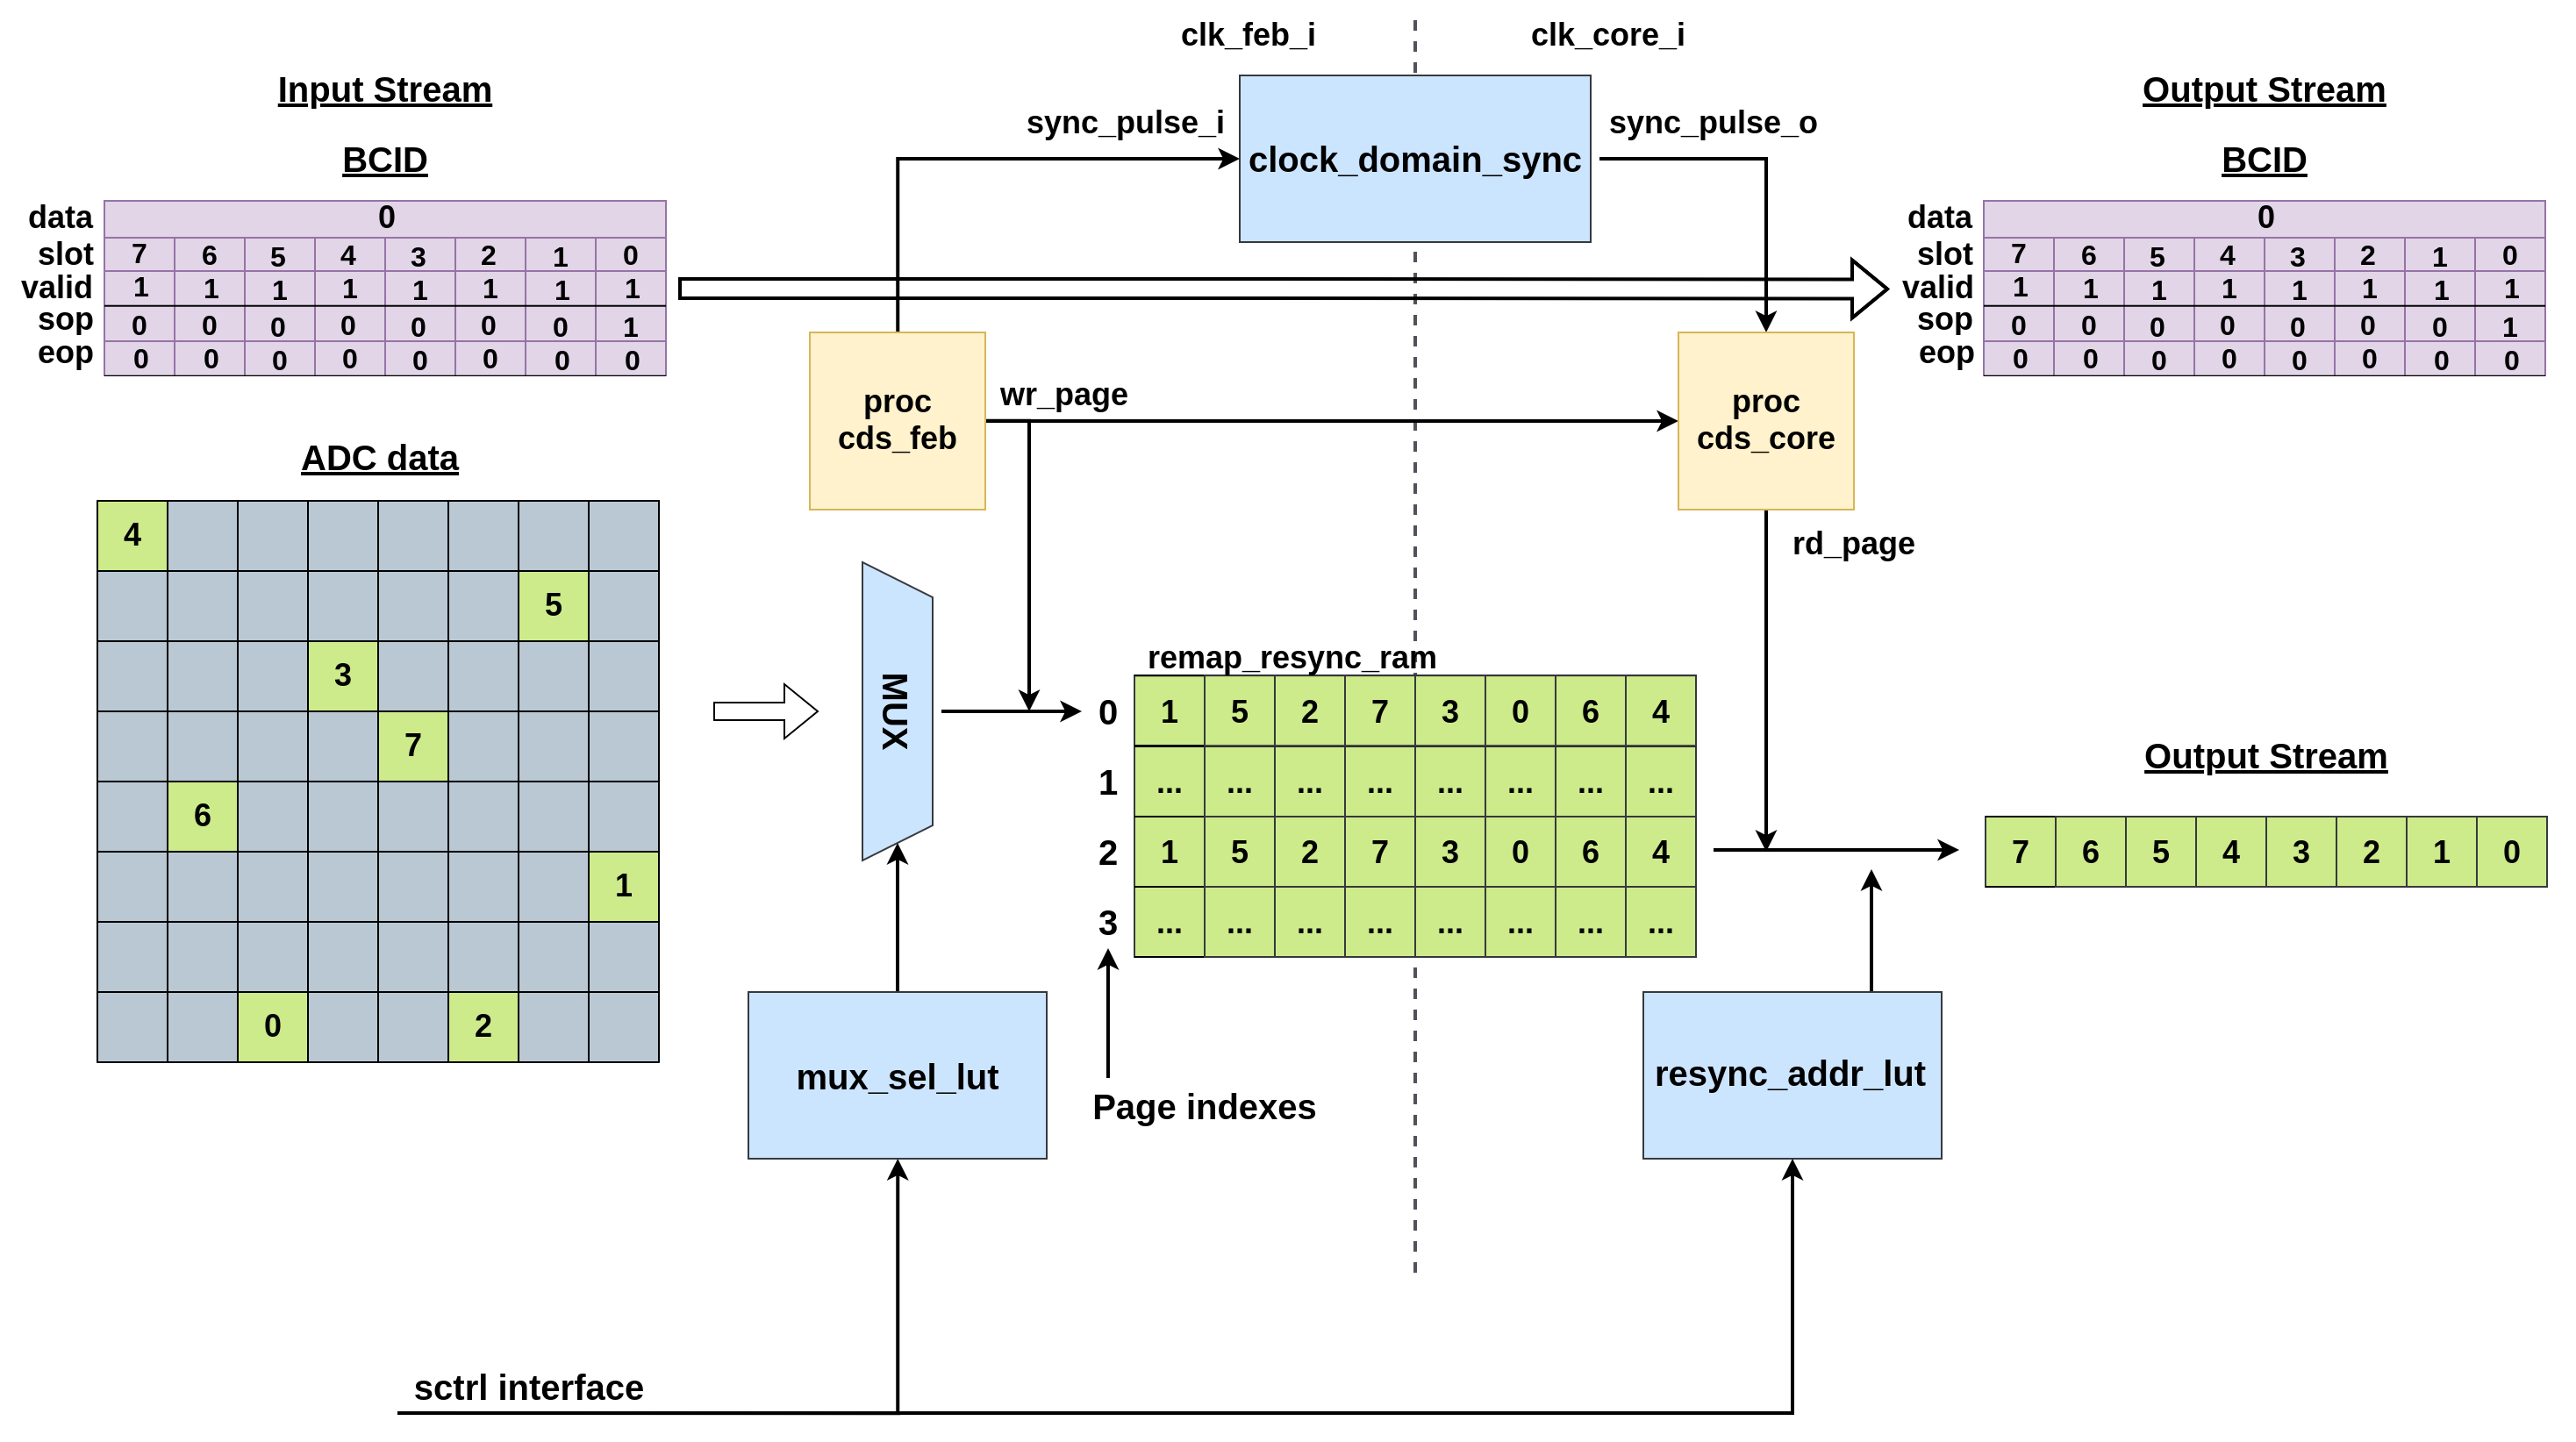
\includegraphics[width=\linewidth]{remap_cds.png}
    \caption{Схема архитектуры модуля \texttt{remap} с модулем синхронизации тактовых доменов ПЕРЕВЕСТИ}
    \label{fig:remap_cds}
\end{figure}\par
Основной особенностью этой архитектуры является то, что в качестве буфера для мультиплексированных данных используется блок двухпортовой RAM памяти. Эта память разбита на несколько страниц, каждая из которых имеет размер, достаточный для хранения захваченной информации, относящейся к одному столкновению пучков. Чтение данных из страницы начинается лишь только после её полного заполнения записывающей стороной. Для синхронизации процессов считывания и записи предусмотрен следующий механизм: по завершению заполнения страницы памяти записывающая логика генерирует импульс шириной в один такт и отправляет его на вход специального модуля. Внутри этого модуля расположены два счётчика, работающие на тактовых частотах $f_{feb}$ и $f_{core}$, которые ведут счёт в диапазоне количества временных ячеек для каждого BCID. В рабочем режиме первый настроен так, чтобы обнуляться одновременно с поступлением синхросигнала от записывающей логики, а второй с задержкой около такта $f_{feb}$ после первого. При завершении цикла работы второго счётчика формируется выходной сигнал синхронизации, который поступает к считывающей логике и означает, что очередная страница в двухпортовой памяти заполнена полностью и можно безопасно извлекать из неё данные. При сбое синхронизации синхросигнал от системы записи придёт не вовремя, модуль это обнаружит и перейдёт в режим восстановления синхронизации. Часть данных после сбоя синхронизации будет утеряно, но через некоторое время система модуля автоматически восстановится и продолжит работать исправно.\par
Описанная архитектура была реализована на языке описания цифровой логики VHDL и отлажена. По результатам тестирования в симуляторе она подтвердила свою работоспособность. Однако такой подход имеет ряд недостатков, главным из которых является необходимость передавать целый набор сигналов(такие как номер текущей страницы, индекс столкновения пучка, а также ряд вспомогательных сигналов внутри модуля синхронизации тактовых доменов) между тактовыми доменами $f_{feb}$ и $f_{core}$ вручную, используя схемы на двух регистрах. Для корректной организации таких переходов требуется тонкая ручная настройка временных ограничений, реализуемая путём составления специальных указаний синтезатору физической схемы, входящему в состав программного комплекса Intel Quartus Prime. Это значительно усложняет весь проект и делает его гораздо менее гибким. После возникновения проблем с разводимостью логики проекта LATOME \parencite{latome}, который является основой задетекторной электроники эксперимента ATLAS, разработанной в рамках предшествующей фазы обновления детектора, командой разработчиков сигнального процессора LASP было принято решение максимально избегать подобные способы перехода между тактовыми доменами. Кроме того, данный вариант является довольно путанным и сложным для понимания в деталях. Учитывая все эти недостатки, было решено разработать альтернативную архитектуру модуля \texttt{remap}.\par
